%= local definitions of macros ============================
\newcommand{\Herwig}{H\protect\scalebox{0.8}{ERWIG}\xspace}
\newcommand{\Pythia}{P\protect\scalebox{0.8}{YTHIA}\xspace}
\newcommand{\Sherpa}{S\protect\scalebox{0.8}{HERPA}\xspace}
\newcommand{\Rivet}{R\protect\scalebox{0.8}{IVET}\xspace}
\newcommand{\Professor}{P\protect\scalebox{0.8}{ROFESSOR}\xspace}
\newcommand{\eps}{\varepsilon}
\newcommand{\mc}[1]{\mathcal{#1}}
\newcommand{\mr}[1]{\mathrm{#1}}
\newcommand{\mb}[1]{\mathbb{#1}}
\newcommand{\tm}[1]{\scalebox{0.95}{$#1$}}
\newcommand{\SMEFTsim}{\texttt{SMEFTsim}}
\newcommand{\SMEFTatNLO}{\texttt{SMEFT@NLO}}
\newcommand{\Madgraph}{M\protect\scalebox{0.8}{ADGRAPH}\xspace}
%= title + authors =====================================
\section{Study of EFT effects in loop induced Higgs processes ~\protect\footnote{
  A.~Cueto,
  S.~Pigazzini}{}}

%= MANDATORY label ======================================
\label{sec:projname}

%= (optional) preamble ================================== 
%\begin{abstract}

%\end{abstract}

%= content ===== ========================================
\subsection{Introduction}
\label{sec:higgseft:section1}
The Standard Model Effective Field Theory (SMEFT) approach is a powerful tool to look for hints of new physics. It allows to study large sets of experimental data without assuming that the theory used is valid to arbitrarily high energies. In the SMEFT, the Standard Model (SM) as we know it is just an effective theory at energies around the electroweak scale. Beyond the Standard Model (BSM) physics manifests at higher scales, $\Lambda$, and is parameterised in terms of higher-dimmensional operators that conserve the same fields and symmetries as the SM. At any mass dimension, a complete bases of non-reduntant operators can be worked out and the full Lagrangian can be written as a power expansion
\begin{equation}
\mathcal{L}_{\textrm SMEFT} = \mathcal{L}_{\textrm SM} + \sum_{d>4}\sum_{i}\frac{c_i}{\Lambda^{d-4}}\mathcal{O}_{i}^{(d)},
\end{equation}  

where $\mathcal{L}_{\textrm SM}$ is the SM Lagrangian, $c_i$ are the Wilson coefficients and ${\mathcal{O}^{d}}$ the set of independent operators for dimension $d$. Operators with $d=5,7$  violate lepton and/or baryon number conservation~\cite{Degrande:2012wf,Kobach:2016ami}. Thus, dimension-6 operators represent the leading deviation from the SM and will be the focus of this work. The modification of a cross section by the insertion of one dimesion-6 operator in the amplitudes can be written as

\begin{equation}
\sigma = \sigma_{\textrm SM} + \sum_{i}\sigma_i^{\textrm int} \frac{c_i}{\Lambda^{2}} + \sum_{i,j}\sigma_{(i,j)}^{\textrm BSM} \frac{c_ic_j}{\Lambda^{4}},
\end{equation}  

where $\sigma_{\textrm SM}$ is the SM cross section of a given process, $\sigma_i^{\textrm int}$ is the interference between the SM and BSM amplitudes and $\sigma_{(i,j)}^{\textrm BSM}$ represents the pure BSM correction to the SM cross section. The leading term is formally $\sigma_i^{\textrm int}$ and the one than will be investigated in this work. 

Several bases of independent operators can be found in the literature~\cite{Grzadkowski:2010es,Contino:2013kra,Gupta:2014rxa,Masso:2014xra}. In the context of the study of the Higgs boson, the SILH basis~\cite{Contino:2013kra} has been commonly used. However, it is not optimised for, for example, diboson processes. Even if the translation between bases is known and has been automated~\cite{Falkowski:2015wza,Aebischer:2017ugx}, experimental collaboration have started to publish their EFT interpretations in the Warsaw basis also in the Higgs sector~\cite{ATLAS:2019jst,ATL-PHYS-PUB-2019-042} to facilitate future global fits of electroweak, Higgs and top data.

The procedure to test the EFT effects for a given set of measurements can be tedious in practice and a big effort has been devoted to develop public code to perform this task in a automatic and generic way~\cite{Brivio:2019irc}. For the Warsaw basis, different Universal FeynRules Output (UFO)~\cite{Degrande:2011ua} models are available which can be interfaced with modern event generators.

The \SMEFTsim\ code~\cite{Brivio:2017btx} is a well documented UFO implementation of the full set of dimension-6 operators in the Warsaw basis. Its main scope is the estimation of the leading SMEFT corrections to the SM. The effective Lagrangian is truncated at $\Lambda^{-2}$ and not supported for next-to-leading-order (NLO) simulations. For Higgs data interpretation the model have become of common use due to its completeness~\cite{Ellis:2018gqa,ATLAS:2019jst}.  To reproduce all the main Higgs production and decay channels in the SM, the loop-induced processes ($hgg$, $h\gamma\gamma$,$hZ\gamma$) are included as effective vertices. However, this implementation might not result satisfactory for reasons as the ones exposed below:
\begin{itemize}
\item Only operators with the same point-like structure as the effective vertices included to reproduce loop-induced processes can modify the cross sections of these processes. That means that, for example, a modification of the top Yukawa will not affect the gluoon-gluon fusion Higgs production process.
\item Given the truncation of the Lagrangian, operators that enter in the shifts to input parameters and that will modify the cross section of any tree-level process does not modify the cross section of loop-induced processes.
\item A reliable computation of the Higgs plus jet  production in gluon-gluon fusion requires top quark loop amplitudes at high $p_{\textrm T}$ and the implementation of $gggH$ vertices.
\item The $gg\to ZH$ process cannot be simulated.
\end{itemize}

To overcome these concerns the \SMEFTatNLO\ tool~\cite{SMEFTNLO} can be used for the loop induced Higgs processes. The tool includes a complete implemation of the SMEFT compatible with NLO QCD predictions. In this work, we study the $gg\to ZH$ and $gg\to H$ processes using this tool. 







\subsection{Comparison between models}
\label{sec:higgseft:section2}
The \SMEFTsim\ and \SMEFTatNLO\ tools have been validated against each other~\cite{Durieux:2019lnv} for the top sector. In this section we compare both models at leading order (LO) by checking the cross sections of the $pp\to ZH$ and $pp\to t\bar{t}H$ processes. The comparison is made at the cross section level and, thus, not expected to be in perfect agreement since it will be affected by phase-space integration. The main goal of this comparison is to show the mapping between the different Wilson coefficients naming and to ensure that the setup used for both models is consistent.

For both models we use the $m_Z$, $m_W$, $G_F$ scheme of electroweak parameters\footnote{We use the \texttt{SMEFTsim\_A\_U35\_MwScheme\_UFO} model for \SMEFTsim\ and the \texttt{SMEFTatNLO\_U2\_2\_U3\_3\_cG\_4F\_LO\_UFO-LO} model for \SMEFTatNLO\ }. The latest versions of the models available in December 2020 is used.  The \Madgraph 2.6.6 generator is used to obtain the cross sections results. The definition of the processes is as follows for the SM results:

\noindent
{\bf ttH:}\\
\noindent
  \texttt{ define p = p b b$\sim$ }\\
  \texttt{ generate p p $>$ h t t$\sim$ SMHLOOP=0 NP=0 }

\noindent
{\bf ZH:}\\
  \noindent
  \texttt{ define p = p b b$\sim$} \\
  \texttt{ generate p p $>$ h l+ l- SMHLOOP=0  NP=0     }\\
  
  The values of several parameters like $m_W$, $mt$, $\alpha_S$ or $\Gamma H$ differ in the default settings of the models and they were set to the same values.

  The tables below show the comparison between the predictions obtained for SM in both models as well as the interference terms, obtained with the NP$^{\wedge}$2$==$1 (NP$^{\wedge}$2$==$2)  for the \SMEFTsim\ (\SMEFTatNLO\ ) model.

  \begin{table}[h]
    \centering
    \resizebox{\columnwidth}{!}{% 
    \begin{tabular}{|l|l|c|c|}
      \hline
      \textbf{Operator} &\textbf{W. coefficient} & \textbf{SMEFTsim} & \textbf{SMEFTatNLO} \\
      \hline 
      &  SM-SM & 0.0251$\pm$ 0.0001& 0.0255$\pm$ 0.0003\\
      \hline 
      $(H^{\dagger}H)\square((H^{\dagger}H)$ & cHbox-cpd & 0.00304$\pm$ 0.00001& 0.00308 $\pm$ 0.00003\\
      \hline
      $\left(H^\dag D^\mu H\right)^* \left(H^\dag D_\mu H\right)$ & cHDD-cpDC & 0.00041$\pm$ 0.00001& 0.00043$\pm$ 0.00006\\
      \hline 
      $ H^\dag H\, B_{\mu\nu} B^{\mu\nu}$ & cHB-cpBB & 0.00231$\pm$ 0.00001& 0.00229$\pm$ 0.00004\\
      \hline
      $H^\dag H\, W^I_{\mu\nu} W^{I\mu\nu}$ & cHW-cpW & 0.01818$\pm$ 0.00007& 0.0183$\pm$ 0.0002\\
      \hline 
      $ H^\dag \tau^I H\, W^I_{\mu\nu} B^{\mu\nu}$ &cHWB-cpWB & 0.00838$\pm$ 0.00004& 0.0084$\pm$ 0.0001\\
      \hline 
      $(H^\dag i\overleftrightarrow{D}_\mu H)(\bar d_p \gamma^\mu d_r)$ & cHd-cpd &-0.0044$\pm$ 0.0002 & -0.00444$\pm$ 0.00004\\
      \hline
      %cHq3-c3pqi & 0.049$\pm$ 0.001& 0.0478$\pm$ 0.0005\\
      %\hline
      $(H^\dag i\overleftrightarrow{D}_\mu H)(\bar e_p \gamma^\mu e_r)$ & cHe-(cpe+cpmu) &-0.002853$\pm$ 0.000007& -0.00285$\pm$ 0.00001\\
      \hline
      $(H^\dag i\overleftrightarrow{D}_\mu H)(\bar l_p \gamma^\mu l_r)$ & cHl1-(cpl1+cpl2) & 0.00324$\pm$ 0.00002 & 0.00327$\pm$ 0.00002\\
      \hline
      $(H^\dag i\overleftrightarrow{D}^I_\mu H)(\bar l_p \tau^I \gamma^\mu l_r)$ & cHl3-(c3pl1+c3pl2) & -0.00588$\pm$ 0.00002& -0.00590$\pm$ 0.00005\\
      
      \hline
    \end{tabular}
}    
    \caption{ Comparison of the SM and interference predicitions for the Z($l^{+}l^{-}$)H process between the \SMEFTsim\ and \SMEFTatNLO\ }

  \end{table}






\begin{center}
  \begin{table}[h]
    \resizebox{\columnwidth}{!}{% 

\begin{tabular}{|l|l|c|c|}
\hline
\textbf{Operator}& \textbf{W. coefficient} & \textbf{SMEFTsim} & \textbf{SMEFTatNLO} \\
 \hline
 &  SM-SM & 0.402$\pm$ 0.001& 0.402$\pm$ 0.003\\
 \hline
$(H^{\dagger}H)\square((H^{\dagger}H)$  & cHbox-cpd & 0.049$\pm$ 0.001 & 0.04876$\pm$ 0.00002\\
 \hline
$ \left(H^\dag D^\mu H\right)^* \left(H^\dag D_\mu H\right)$ & cHDD-cpDC & -0.01218$\pm$ 0.00002 & -0.01222$\pm$ 0.00008\\
 \hline
 $ H^\dag H\, B_{\mu\nu} B^{\mu\nu}$ & cHB-cpBB & 0.0000893$\pm$ 0.0000002 & 0.0000897$\pm$ 0.0000008\\
 \hline
$H^\dag H\, W^I_{\mu\nu} W^{I\mu\nu}$ & cHW-cpW & 0.00042$\pm$ 0.000001& 0.000423$\pm$ 0.000004\\
 \hline
$ H^\dag \tau^I H\, W^I_{\mu\nu} B^{\mu\nu}$ &  cHWB-cpWB & -0.0002499$\pm$ 0.0000005& -0.000253$\pm$ 0.000002\\
 \hline
$(H^\dag i\overleftrightarrow{D}_\mu H)(\bar d_p \gamma^\mu d_r)$ & cHd-cpd & -0.0000761$\pm$ 0.0000003 & -0.000076$\pm$ 0.000002\\
 \hline
% cHq3-c3pqi & 0.20976E-02$\pm$ 0.56257E-05& 0.12428E-02$\pm$ 0.17784E-04\\
% \hline
$(H^\dag H)(\bar q_p u_r \widetilde H )$ & cuHAbs-ctp & -0.0488$\pm$ 0.0001& -0.0494$\pm$ 0.0003\\
 \hline
$(\bar q_p \sigma^{\mu\nu} T^A u_r) \widetilde H \, G_{\mu\nu}^A$ & cuGAbs-ctG & -0.3393$\pm$ 0.0009 & 0.407 $\pm$ 0.002\\
% \hline
%$(\bar q_p \sigma^{\mu\nu} u_r) \widetilde H \, B_{\mu\nu}$ & cuBAbs-ctZ & -0.00083$\pm$ 0.000002 & -0.00175$\pm$ 0.00002\\
% \hline
%$(\bar q_p \sigma^{\mu\nu} u_r) \tau^I \widetilde H \, W_{\mu\nu}^I$ &cuWAbs-ctW & -0.002219$\pm$ 0.000006& 0.00378$\pm$ 0.00003\\
% & cuBAbs-ctB & -0.82828E-03$\pm$ 0.20643E-05& 0.84754E-03$\pm$ 0.10257E-04\\
% \hline
% & cuWAbs-ctW & -0.22186E-02$\pm$ 0.63027E-05& 0.22314E-02$\pm$ 0.22095E-04\\
  \hline
 $(H^\dag i\overleftrightarrow{D}^I_\mu H)(\bar l_p \tau^I \gamma^\mu l_r)$  & cHl3-(c3pl1+c3pl2) & -0.0489 $\pm$ 0.0001 & -0.0491 $\pm$ 0.0002\\
 \hline
\end{tabular}
}
\caption{ Comparison of the SM and interference predicitions for the ttH process between the \SMEFTsim\ and \SMEFTatNLO\ .}
\end{table}
\end{center}

In the tables, $H$ is the SU$_{\textrm L}$(2) scalar doublet. The gauge covariant derivative is defined as  $D_\mu = \partial_\mu + i g_3 T^A A^A_\mu + i g_2  t^I W^I_\mu + i g_1 y B_\mu$, where $T^A$ are the $\rm SU_c(3)$ generators, $t^I=\tau^I/2$ are the $\rm SU_L(2)$ generators, and $y$ is the $\rm U_Y(1)$ hypercharge. The fields $\{q,l \}$ are left handed and the fields $\{e,u,d\}$ are right handed. The definition $\sigma_{\mu \, \nu} = i \, [\gamma_\mu,\gamma_\nu]/2$ is used. The subscripts $p,r,s$ and $t$ are flavour indices.

For the ttH production mode differences are observed for the ctG operator. These differences are acknowledged by the authors of the models and reside in the absence of five-point interactions and higher in the \SMEFTsim model. It will be corrected in future versions of the model.

For the $\mathcal{O}_uW$ and $\mathcal{O}_uB$ operators defined as,

$$ \mathcal{O}_uB = (\bar q_p \sigma^{\mu\nu} u_r) \widetilde H \, B_{\mu\nu}; \quad
   \mathcal{O}_uW =  (\bar q_p \sigma^{\mu\nu} u_r) \tau^I \widetilde H \, W_{\mu\nu}^I
$$

   there is no one-to-one correspondence between the models in their latest versions. The \SMEFTatNLO\ version released on 2019/04/03 was used instead to compare these two operators.

\begin{center}
  \begin{table}[h]
    \resizebox{\columnwidth}{!}{%  
      \begin{tabular}{|l|l|c|c|}
        \hline
        \textbf{Operator}& \textbf{W. coefficient} & \textbf{SMEFTsim} & \textbf{SMEFTatNLO} \\
        \hline
        \hline                                                                                                                                              
        $(\bar q_p \sigma^{\mu\nu} u_r) \widetilde H \, B_{\mu\nu}$ & cuBAbs-ctB & -0.000828$\pm$ 0.000002 &-0.00085$\pm$ 0.00001 \\
         \hline
        $(\bar q_p \sigma^{\mu\nu} u_r) \tau^I \widetilde H \, W_{\mu\nu}^I$ &cuWAbs-ctW & -0.002219$\pm$ 0.000006& 0.00223$\pm$ 0.00002\\
        \hline
 
\end{tabular}
    }
    \caption{ Comparison of the SM and interference predicitions for the ttH process between the \SMEFTsim\ and \SMEFTatNLO\ for |cuB| (ctB) and |cuW| (ctW). The operator definition are given in the way they are implemented in \SMEFTsim\ .}
    \label{tab:higgseft:comptth2}
\end{table}
\end{center}

The prediction for the operators shown in Table~\ref{tab:higgseft:comptth2} agree in their absolute value but not in their sign. The way in which they are implemented in the model is also different. While in \SMEFTsim\ the absolute value and the phase of these complex operators can be changed by the user, only the real part can be tuned by the user in \SMEFTatNLO.

Other differences come from two-fermion operators involving quarks. In \SMEFTsim\ the couplings of all quarks enter equally, while in \SMEFTatNLO\ the top vertices are parameterized separately. 


\subsection{$gg\to ZH$}
\label{sec:higgseft:ggzh}
The study of  $gg\to Z(l^{+}l^{-})H$ was performed using the \SMEFTatNLO\ model. The renormalization and factorization scales were set to $M_H=125$~GeV and the PDF set NNPDF2.3 for the parametrisation of the proton structure. A more in depth study of the SMEFT effects for this process was performed in~\cite{Bylund:2016phk} using the main set of operators affecting the cross sections using merged samples of up to one additional parton. Here we have considered all the operators available at NLO in \SMEFTatNLO\ which provide diagrams with a non-zero interference with the SM.

In Figure~\ref{fig:higgseft:ggzh}, differential distributions as functions of $p_{T}^{V}$ and $m_{HV}$ are shown. The BSM effects caused by cp3qi, cpu, ctG and ctp~\footnote{The definition of these operators can be seen in~\cite{SMEFTNLOdefs}} is shown.  Many other operators modify the cross section of this process but only some examples of those that distort significantly the shape of the SM prediction for  $c_i=1$ are shown.

\begin{figure}
\includegraphics[width=0.49\linewidth,page=7]{figures/kinematics_ggHll_np0.pdf}
\includegraphics[width=0.49\linewidth,page=10]{figures/kinematics_ggHll_np0.pdf}
\label{fig:higgseft:ggzh}
\caption{Differential distributions as a function of $p_{T}^{V}$ and $m_{HV}$ for the SM predictions and its interference with operators with Wilson coefficients ctG, cpd, cpu and ctp  at the lowest order in QCD. The value of $\Lambda$ was set to 1 TeV}  
\end{figure}

In addition to differential cross sections, measurements  of the Higgs couplings in terms of Simplified Template Cross Sections (STXS)~\cite{deFlorian:2016spz} also provide constraining power of the SMEFT parameters. A parametrisation in bins of the STXS in stage 1.2~\cite{Berger:2019wnu}  for $gg\to Z(l^{+}l^{-}H$  is provided in Table~\ref{tab:higgseft:stxsggzh}.

\begin{table}[h!]
 \adjustbox{max width=\textwidth}{
  \begin{tabular}{p{0.40\textwidth} p{0.60\textwidth}}
    \toprule


      \hline
      \textbf{Bin} & Parametrization \\
      \hline 
    $gg\to Hll (p_{\textrm T}^{V}<75$~GeV)&
     -0.0012 cpDC +0.121 cdp -0.056 cpe +0.064 cpl1 +0.064 cpl2 -0.0566 cpmu -0.331 cpq3i -0.117 c3pl1 -0.117 c3pl2 +0.249 cpd -0.166 cpQ3 -0.129 cpQM -0.332 cpqMi +0.047 cpt +0.165 cpu +0.250 ctG +0.0369 ctp  \\
     \hline 
     $gg\to Hll (75<p_{\textrm T}^{V}<150$~GeV)&
     +0.0030 cpDC +0.122 cdp -0.057 cpe +0.065 cpl1 +0.065 cpl2 -0.0568 cpmu -0.285 cpq3i -0.118 c3pl1 -0.118 c3pl2 +0.213 cpd -0.142 cpQ3 -0.098 cpQM -0.283 cpqMi +0.0262 cpt +0.142 cpu +0.316 ctG +0.0454 ctp\\
     \hline
     $gg\to Hll $(0-jet,$150<p_{\textrm T}^{V}<250$~GeV)&
     +0.025 cpDC +0.120 cdp -0.057 cpe +0.065 cpl1 +0.065 cpl2 -0.0561 cpmu -0.233 cpq3i -0.116 c3pl1 -0.118 c3pl2 +0.17 cpd -0.115 cpQ3 -0.029 cpQM -0.229 cpqMi -0.027 cpt +0.112 cpu +0.439 ctG +0.084 ctp  \\
     \hline
     $gg\to Hll (\geq$ 1-jet,$150<p_{\textrm T}^{V}<250$~GeV)&
 +0.016 cpDC +0.122 cdp -0.0569 cpe +0.065 cpl1 +0.065 cpl2 -0.0572 cpmu -0.244 cpq3i -0.118 c3pl1 -0.117 c3pl2 +0.183 cpd -0.122 cpQ3 -0.050 cpQM -0.245 cpqMi -0.0111 cpt +0.121 cpu +0.411 ctG +0.072 ctp  \\
 \hline

      $gg\to Hll (p_{\textrm T}^{V}>250$~GeV)&
 +0.049 cpDC +0.120 cdp -0.0585 cpe +0.066 cpl1 +0.066 cpl2 -0.0581 cpmu -0.197 cpq3i -0.116 c3pl1 -0.116 c3pl2 +0.153 cpd -0.099 cpQ3 +0.031 cpQM -0.199 cpqMi -0.0820 cpt +0.099 cpu +0.544 ctG +0.134 ctp \\
 \bottomrule
\end{tabular}
}

\caption{Parametrization of the $gg\to ZH$ bins of the STXS as defined in its stage 1.2 with the parameters definitions of the \SMEFTatNLO\ model}

\end{table}

\subsection{$gg\to H$}
\label{sec:higgseft:section3}
The SMEFT effects in the Higgs production through gluon-gluon fusion is examined using the \SMEFTatNLO\ package. As in Section~\ref{sec:higgseft:ggzh}, the 
study of this process is already available in the literature~\cite{Deutschmann:2017qum} for a limited set of operators. In this work we have considered all operators that have a non-zero interference with the SM. Those operators were found to be:
%$\mathcal{O}_{\textrm \phi G}$, $\mathcal{O}_{\textrm tG}$, $\mathcal{O}_{\textrm tp}$, $\mathcal{O}_{\textrm dp}$, $\mathcal{O}_{\textrm pDC}$, $\mathcal{O}_{\textrm \phi l1}^{(3)}$ and $\mathcal{O}_{\textrm \phi l2}^{(3)}$.
The last four operators enters in the process though shifts to the inputs parameters and dot modify the shape of the SM predictions.


 \textcolor{red}{ SETUP, check with Simone}


  
 \textcolor{red}{PLOTS}

  

 In Table~\ref{tab:higgseft:stxsggh}, we provide the parametrisation of the $gg\to H$ STXS bins in stage 1.2.

 
 \textcolor{red}{ Parametrization for 0-jet and 1-jet still missing}
 
\begin{table}[h!]
 \adjustbox{max width=\textwidth}{
  \begin{tabular}{p{0.40\textwidth} p{0.60\textwidth}}
    \toprule


      \hline
      \textbf{Bin} & Parametrization \\    
      $gg\to H$ ($\geq$ 2-jet, $m_{\textrm jj}<350$~GeV, $p_{\textrm T}^{H}<60$~GeV)&
      1.62 ctG -0.061 c3pl1 -0.061 c3pl2 +0.126 cdp -0.031 cpDC -0.122 ctp +41 cpG \\
      \hline
      $gg\to H$ ($\geq$ 2-jet, $m_{\textrm jj}<350$~GeV, $60<p_{\textrm T}^{H}<120$~GeV)&
      +1.63 ctG -0.061 c3pl1 -0.061 c3pl2 +0.120 cdp -0.031 cpDC -0.121 ctp +40.8 cpG  \\
      \hline
      $gg\to H$ ($\geq$ 2-jet, $m_{\textrm jj}<350$~GeV, $120<p_{\textrm T}^{H}<200$~GeV)&
      +1.69 ctG -0.062 c3pl1 -0.062 c3pl2 +0.120 cdp -0.030 cpDC -0.122 ctp +45 cpG  \\
      \hline
      $gg\to H$ ($\geq$ 2-jet, $350<m_{\textrm jj}<700$~GeV, $p_{\textrm T}^{H}<200$~GeV, $p_{\textrm T}^{Hjj}<25$~GeV)&
      +1.5 ctG -0.056 c3pl1 -0.056 c3pl2 +0.113 cdp -0.027 cpDC -0.113 ctp +42 cpG \\
      \hline
      $gg\to H$ ($\geq$ 2-jet, $350<m_{\textrm jj}<700$~GeV, $p_{\textrm T}^{H}<200$~GeV, $p_{\textrm T}^{Hjj}>25$~GeV)&
      
      +1.60 ctG -0.060 c3pl1 -0.060 c3pl2 +0.117 cdp -0.028 cpDC -0.126 ctp + 40 cpG  \\
      \hline
      $gg\to H$ ($\geq$ 2-jet, $m_{\textrm jj}>700$~GeV, $p_{\textrm T}^{H}<200$~GeV, $p_{\textrm T}^{Hjj}<25$~GeV)&  
      +1.7 ctG -0.058 c3pl1 -0.058 c3pl2 +0.12 cdp -0.033 cpDC -0.12 ctp +48 cpG  \\
      \hline
      $gg\to H$ ($\geq$ 2-jet, $m_{\textrm jj}>700$~GeV, $p_{\textrm T}^{H}<200$~GeV, $p_{\textrm T}^{Hjj}>25$~GeV)&  
      +1.7 ctG -0.062 c3pl1 -0.062 c3pl2 +0.114 cdp -0.031 cpDC -0.118 ctp +44 cpG \\
      \hline

       \bottomrule
\end{tabular}
}

\caption{Parametrization of the $gg\to H$ bins of the STXS as defined in its stage 1.2 with the parameters definitions of the \SMEFTatNLO\ model}
\label{tag:higgseft:stxsggh}
\end{table}
    
    
The parametrization of cpG for the $gg\to H$ production mode is different in the \SMEFTsim\ and \SMEFTatNLO\ . It has been checked that for the 0-jet case the values of the inclusive cross section in those models is the same. In this case, the same SMEFT effects are observed. However, when we add jets to the final state, the parametrization changes significantly (it can be compared to the one shown in~\cite{ATL-PHYS-PUB-2019-042}). This is expected due to the different implementation of the process and different diagrams included.


\subsection{Summary and conclusions}
In the absence of hints for new physics in the LHC, the SMEFT approach started to be widely adopted by the experimental collaborations for the interpretation of their measurements. In order to be able to have predictions for the SMEFT, implementation of the SM plus dimension-6 Lagrangian in form of UFO files that can be interfaced with modern event generators are needed. Two different tools: \SMEFTsim\ and \SMEFTatNLO\ has been used and compare to study the $gg\to H$ and $gg\to ZH$ loop-induced processes. For the former, which is mainly meant for performing LO calculations, the $gg\to ZH$ process cannot be simulated and only one-loop functions for $gg\to H$ are implemented. It lacks, for example, of $gg\to Hg$ one loop-function exists making the calculation of Higgs plus jets unreliable. It also truncates the Lagrangian for contributions that have a loop supression on top of the $\Lambda^{-2}$.

In this work we have compared both tools for the ttH and ZH production processes. The agreement between the predictions for the SM and interference terms is excellent except for the $\mathcal{O}_{\textrm tG}$ operator. Some other operators like $\mathcal{O}_{\textrm tW}$, $\mathcal{O}_{\textrm tZ}$, or two-fermion currents involving quarks cannot be directly compared. It would be helpful for the user to to have a clear mapping between each operator in both models.

The SMEFT effects have been studied by means of the distortion of the SM prediction shape and normalization in differential cross sections as well as the parametrization of STXS bins. Only the interference effects have been shown. For $gg\to H$
\textcolor{red}{Fill with conclusions of the plots}
The parametrisation in terms of STXS bins for $\mathcal{O}_{\phi G}$ differs from others that can be found in the literature using \SMEFTsim\ due to the differences in the implementation of this process in both tools.
For $gg\to ZH$, with $Z\to l^{+}l^{-}$,  many operators change the cross sections. However, most of them just introduce a deviation in the normalization of the SM predictions at the interference level whithout distorting the SM shape. Among the ones that have an energy dependence we can find: $\mathcal{O}_{tG}$,...

The use of \SMEFTsim\ for EFT interpretations of Higgs measurements can result insatisfactory for Higgs loop-induced processes. In this cases, as we have shown, the \SMEFTatNLO\ tool can be used instead. The NLO effects on the decays have not been studied here. This work could have been extended with studies of $H\to \gamma\gamma$ and $ H\to Z\gamma$. They exist in the literature~\cite{Dawson:2018liq} for $H\to \gamma\gamma$. However, none of the tools are able to provide the NLO QED corrections for these processes in the SMEFT.



~\newline~

%= undefine macros (MANDATORY) ====================
\let\Herwig\undefined
\let\Pythia\undefined
\let\Sherpa\undefined
\let\Rivet\undefined
\let\Professor\undefined
\let\eps\undefined
\let\mc\undefined
\let\mr\undefined
\let\mb\undefined
\let\tm\undefined




